% Erste Tabelle mit nur der ersten Spalte
\begin{tabular}{|m{0.25\textwidth}|}
    \hline
    \begin{circuitikz}[scale=0.8, transform shape]
        \ctikzset{tripoles/en amp/input height=-0.45}
        \draw (0,0) node[en amp](E){};
        \node at ($(E) + (-1.2, 1.5)$) {\textbf{\LARGE A}}; % Label für den ersten OPV
        \draw (E.out) node[circ]{} node[right]{$U_A$};
        \draw (E.-) node[circ]{} node[left]{0V};
        \draw (E.+) node[circ]{} node[left]{1V};
        \draw (E.up) -- ++(0,0.5) node[anchor=south]{$+U_B$} node[circ] {};
        \draw (E.down) -- ++(0,-0.5) node[anchor=north]{$-U_B$} node[circ] {};
    \end{circuitikz} \\
    \hline
    \multicolumn{1}{|c|}{
    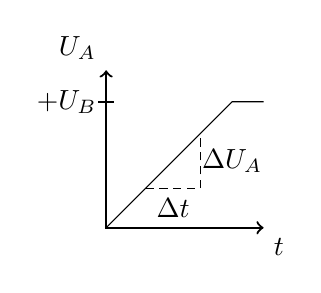
\begin{tikzpicture}
        \draw[thick,->] (-0.015,0) -- (2,0) node[anchor=north west] {$t$};
        \draw[thick,->] (0,0) -- (0,2) node[anchor=south east] {$U_{A}$};
        \draw (0,0) -- (1.6,1.6) -- (2,1.6);
        \draw[thick] (-0.1,1.6) -- (0.1,1.6);
        \draw (0,1.6) node[anchor=east] {$+U_B$};
        
        \draw[densely dashed] (0.5,0.5) -- (1.2,0.5) -- ++(0,0.7);  % Steigungsdreieck Linien
            \node at (1.6,0.85) {$\Delta U_A$};
            \node at (0.85,0.25) {$\Delta t$}; 
    \end{tikzpicture}} \\
    \hline
\end{tabular}